
\section{Zeiger}

Kommen wir nun zu der Frage, wie man aus Funktionen mehr als nur skalare Größen zurück gibt.
Genauso, wie wir Felder an Funktionen uebergeben können, wollen wir auch Felder als Rückgabewert benutzen.
Dies geht in \texttt{C} nicht direkt, sondern nur über den Umweg von sogenannten Zeigern.
Zeiger sind mit das mächtigste Sprachelement in \texttt{C}.
Sie sind allerdings auch für jede Menge Verwirrung und Programmierfehler verantworlich.
\index{Zeiger}

\begin{figure}[h]
  \centering
  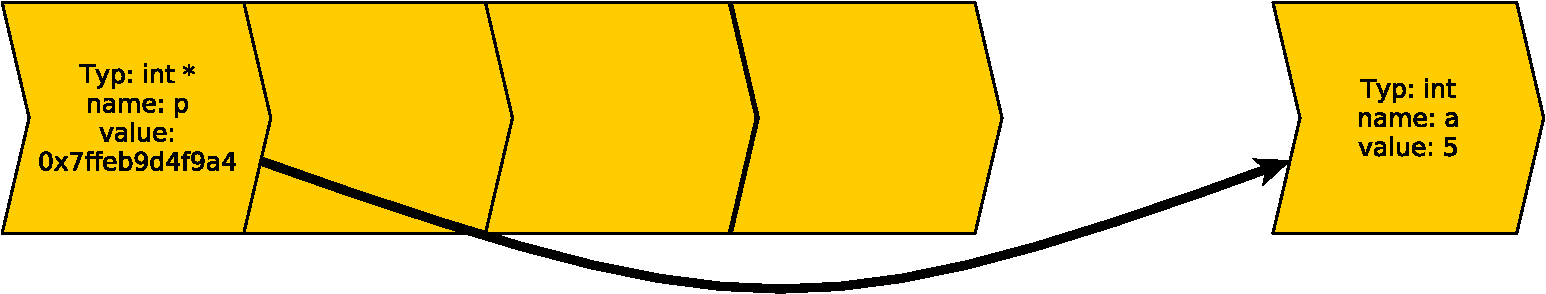
\includegraphics[width=\linewidth]{pointer-crop}
  \caption{\label{pointfig} Illustration Zeiger.}
\end{figure}


Um Zeiger verstehen zu können, muss man sich zunächst noch einmal ins Gedächtnis rufen, das eine Variable im Prinzip aus zwei Dingen besteht:
Einerseits dem Typ der Variablen und andererseits der Speicheradresse, unter der ein Wert abgelegt wird.
Über den Typ der Variablen weiß der Compiler, wie viele Bits im Speicher belegt sind, und wenn die Anfangsadresse für das erste Bit bekannt ist, dann kann die gesamte Anzahl an Bits ausgelesen und entsprechend dem Typ interpretiert werden.
C erlaubt Zugriff sowohl auf den Wert einer Variablen, als auch auf die Adresse, an der der Wert abgelegt ist.
Unterschieden wird zwischen den beiden mit dem \verb|&| Operator.
Für eine Variable \verb|n| repräsentiert \verb|n| den Wert und \verb|&n| die Speicheradresse.
Bei \verb|&n| spricht man auch von Zeiger (\emph{pointer}) und bei \verb|&| vom Adressoperator.\index{Adressoperator}\index{\&}
Mit Hilfe von \texttt{printf} kann man den Unterschied ausgeben
\begin{lstlisting}
  int a = 5;
  int * p = &a;
  printf("Der Wert %d ist an der Adresse %p abgelegt.\n", a, p);
\end{lstlisting}
was eine Ausgabe wie die folgende erzeugt
\begin{verbatim}
  Der Wert 5 ist an der Adresse 0x7ffeb9d4f9a4 abgelegt.
\end{verbatim}
Die Adresse wird hier als \emph{hexadezimal} Zahl \verb|0x7ffeb9d4f9a4| ausgegeben.
Die Beziehung von \verb|p| und \verb|a| ist in Abbildung~\ref{pointfig} illustriert.

Da Zeiger in C eine sehr wichtige Rolle spielt, gibt es für sie spezielle Datentypen, wie im letzten Beispiel schon gesehen:
\begin{lstlisting}
int n = 3; // eine Variable vom Typ int
int *address; // eine Variable vom Typ Zeiger auf int
address = &n; // address zeigt auf n
*address = 5; // *address representiert den Wert, der unter der Adresse address
              // gespeichert ist. man spricht von dereferenzieren
n == 5; // ist jetzt wahr.
\end{lstlisting}
Genauso gibt es einen Typ Zeiger auf \verb|double|, nämlich \verb|double*| und so weiter.
Allgemein ist ein Zeiger eine Variable, die eine als Wert Adresse zusammen mit einem Datentyp speichert.
Wir demonstrieren die Nützlichkeit von Zeigern zunächst an einem Beispiel.
Wir definieren eine Funktion, die zwei Parameter \verb|a, b| übergeben bekommt und diese jeweils um eins erhöht.
Anschließend sollen diese beiden neuen Werte zurückgegeben werden.

Ein Weg, um dies zu tun, ist das sogenannte \emph{call by reference}.
\index{call by reference}
Was \textbf{nicht} funktioniert ist das folgende:
\begin{lstlisting}
#include <stdio.h>
// einfache Funktion um a,b um 1 zu erhoehen
void increment(int a, int b)
{
  a++;
  b++;
  return;
}

int main()
{
  int a = 2, b = 3;
  printf("Wert vor der Funktion a=%d, b=%d\n", a, b);
  increment(a, b); // die Variablen in unserem Block werden
                         // nicht veraendert!
  printf("Wert nach der Funktion a=%d, b=%d\n", a, b);
  return 0;
}
\end{lstlisting}
Der Grund ist, dass in der Funktion \verb|increment| neue Variablen \verb|a|, \verb|b| angelegt werden, die nur in der Funktion selbst sichtbar sind.
Sie haben also nichts mit den Variablen \verb|a|, \verb|b| in der Funktion \verb|main| gemein, außer dem Namen.
Man spricht hier von \emph{call by value}, da die Variablen \verb|a, b| in der Funktion \verb|increment| mit den Werten der Variablen aus \verb|main| initialisiert werden.\index{call by value}
Deswegen liefern die \verb|printf| Aufrufe in den Zeilen 12 und 15 das gleiche Ergebnis.
Denn die Variablen \verb|a|, \verb|b| in \verb|main| wurden nicht verändert.

Bei \emph{call by reference} wird an Stelle des Wertes die Adresse übergeben.\index{call by reference}
\begin{lstlisting}
#include <stdio.h>
// einfache Funktion um a,b um 1 zu erhoehen
void increment(int *a, int *b)
{
  (*a)++;
  (*b)++;
  return;
}

int main()
{
  int a = 2, b = 3;
  printf("Wert vor der Funktion a=%d, b=%d\n", a, b);
  increment(&a, &b); // die Variablen in unserem Block werden
                           // direkt veraendert!
  printf("Wert nach der Funktion a=%d, b=%d\n", a, b);
  return 0;
}
\end{lstlisting}
Die Funktion bekommt also zwei Parameter vom Typ \verb|int*|, also Zeiger auf \verb|int|.
Dann wird mit dem Dereferenzierungsoperator \verb|*| der Wert, der unter den beiden Adressen gespeichert ist, um eins erhöht.
Das geschieht unter der Annahme, dass dort eine Variable vom Typ \verb|int| abgelegt ist.
Damit werden also direkt die Werte der Variable \verb|a, b| in \verb|main| verändert.

Zeiger kann man genau wie andere Variablen nutzen (womit auch klar ist, dass man auch Zeiger auf Zeiger definieren kann).
Folgendes Beispiel illustriert die Nutzung noch einmal, wobei \verb|NULL| der Nullzeiger ist:\index{\texttt{NULL}}
\begin{lstlisting}
#include <stdio.h>

int main()
{
  int q = 10;
  int *p = NULL;
  p = &q;
  printf("Der Wert an der Adresse p ist:%d\n", *p);
  return 0;
}
\end{lstlisting}
In der fünften Zeile haben wir eine Variable vom Typ \verb|int| deklariert und mit dem Wert 10 initialisiert, in der sechsten Zeile eine Variable vom Typ \verb|int*|, die mit dem \verb|NULL| Zeiger initialisiert wurde.
In der siebten Zeile wird dann \verb|p| auf die Adresse von \verb|q| gesetzt.
Damit liefert die Dereferenzierung von \verb|p|, also \verb|*p|, den Wert von \verb|q|.
Zeigern dürfen nur gültige Adressen zugewiesen werden.
Dies kann allerdings, bis auf Ausnahmen, nicht vom Compiler überprüft werden.
Wenn doch keine gültige Adresse zugewiesen wurde, bekommt man bei Dereferenzierung den \emph{segmentation fault} als Laufzeitfehler.\index{segmentation fault}
Dieser Quelltext weist sehr wahrscheinlich eine ungültige Adresse zu:
\begin{lstlisting}
int *p = 42;
\end{lstlisting}
Allerdings wird im diesen Fall der Compiler sehr wahrscheinlich\footnote{Hängt leider vom Compiler ab.} eine Warnung geben, denn 42 ist vom Typ \verb|int|, und nicht vom Typ \verb|int*|.
GCC 6.3.1 gibt folgendes aus:
\begin{verbatim}
int-ptr.c:7:14: Warnung: Initialisierung erzeugt Zeiger 
           von Ganzzahl ohne Typkonvertierung [-Wint-conversion]
     int *p = 42;
              ^~
\end{verbatim}
Wenn der Compiler sich hier nicht beschwert, sollte man die Dokumentation studieren, um heraus zu finden, wie man diesen Typ von Warnung anschalten kann, oder, wenn das nicht möglich ist, den Compiler wechseln.

\subsection{Zeiger und Felder}

\index{Feld}\index{array}
Wie schon im Abschnitt über Felder angedeutet sind Felder und Zeiger in \texttt{C} eng verwandt.
Nehmen wir an, es wurde ein Feld wie oben eingeführt deklariert
\begin{lstlisting}
  int n[] = {1, 2, 3, 4, 5};
\end{lstlisting}
Dann ist die variable \verb|n| vom Typ \verb|int *|, also Zeiger auf \verb|int|.
Das bedeutet, folgendes ist korrekter \texttt{C} Quelltext
\begin{lstlisting}
  int n[] = {1, 2, 3, 4, 5};
  int * p = n;
\end{lstlisting}
und auch die folgenden zwei Funktionsdeklarationen sind äquivalent
\begin{lstlisting}
  void f1(int * a, const int n);
  void f2(int a[], const int n);
\end{lstlisting}
Daraus folgt auch, dass ein Feld in \texttt{C} immer \emph{by reference} übergeben wird.\index{call by reference}
Wird in Funktion \texttt{f1} oder \texttt{f2} in das Feld \texttt{a} geschrieben, so wird das original Feld aus dem aufrufenden Quelltext Block modifiziert.
Obiges Beispiel kann man also auch wie folgt schreiben:
\begin{lstlisting}
  #include <stdio.h>
// einfache Funktion um a,b um 1 zu erhoehen
void increment(int *a, const int n)
{
  for(int i = 0; i < n; i++) {
    a[i]++;
  }
  return;
}

int main()
{
  int a[] = {2, 3};
  printf("Wert vor der Funktion a[0]=%d, a[1]=%d\n", a[0], a[1]);
  increment(a, 2); // die Variablen in unserem Block werden
                           // direkt veraendert!
  printf("Wert nach der Funktion a[0]=%d, a[1]=%d\n", a[0], a[1]);
  return 0;
}
\end{lstlisting}
Wenn das übergebene Feld innerhalb einer Funktion nicht verändert werden soll, so kann man es als \verb|const| deklarieren.\index{\texttt{const}}
Will man nur die Elemente des Feldes konstant lassen, so schreibt man
\begin{lstlisting}
  void f(const int * a, const int n);
\end{lstlisting}


\subsection{Die Parameter der \texttt{main} Funktion}

An dieser Stelle können wir jetzt auch die möglichen Parameter der Funktion \verb|main| einführen.
Die ist nämlich allgemein wie folgt definiert:\index{\texttt{argc}}\index{\texttt{argv}}\index{\texttt{main}}
\begin{lstlisting}
int main(int argc, char *argv[])
{
  return (0);
}
\end{lstlisting}
An der Kommandozeile kann man dem Programm Parameter übergeben.
Die Funktion \verb|main| erhält diese in Form einer Zeichkette.
Leerzeichen in dieser Zeichenkette werden als Trennzeichen interpretiert, so dass die Zeichenkette \verb|argc| Wörter enthält.
Das erste Wort ist immer der Name der Programms.
Die Wörter werden in \verb|argv| gespeichert.
Also, zum Bespiel
\begin{verbatim}
  ./main.exe 3 hallo
\end{verbatim}
liefert \verb|argc=3|, und \verb|argv[0] = "./main.exe"|, \verb|argv[1] = "3"| und \verb|argv[2] = "hallo"|.
\newpage
\begin{myexampleprogram}{Beispiel: \texttt{Näherung von $\pi$}}
  In diesem Beispiel berechnen wir $\pi$ näherungsweise.
  Dafür verwenden wir folgende Integraldarstellung von $\pi$:
  \begin{equation}
    \pi=4\cdot \int_{0}^{1} \mathrm{d}x \dfrac{1}{1+x^2}
  \end{equation}
  Das Integral berechnen wir numerisch, indem wir die Fläche unterhalb der Kurve als eine Summe abschätzen.
  Dabei bedienen wir uns der sogenannten Trapez-Regel.
  Wir teilen das Interval $[0,1]$ in $N$ gleichlange Unterintervalle auf.
  Den jeweilige linke Punkt des Intervals nennen wir $x_i$, $i=0,...,N$, wobei $x_n-x_{n-1}=\Delta=\mathrm{const}$.
  Auf jedem Unterintervall approximieren wir die Funktion linear, wie in folgender Abbildung dargestellt ist:
  \begin{center}
    %\begin{minipage}
    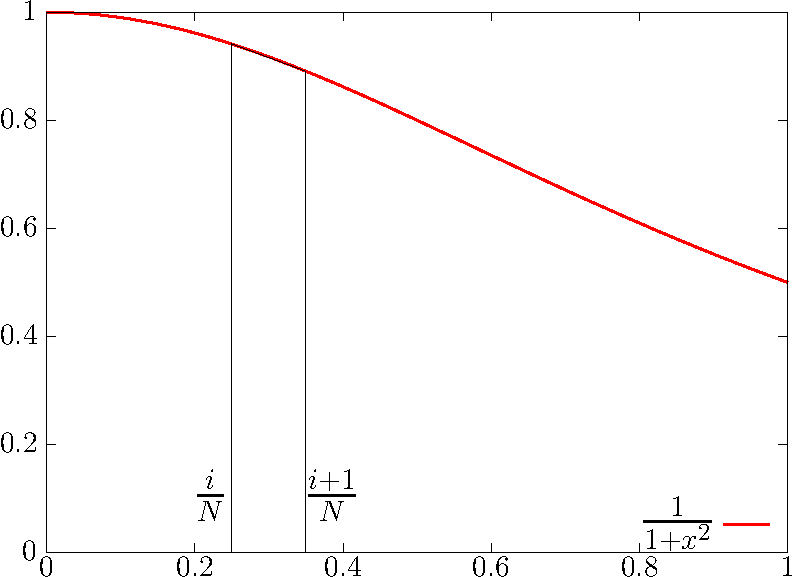
\includegraphics[width=.6\linewidth]{trapez1}
  \end{center}
  In unserem Fall sind die Punkte wie folgt gegeben
  \begin{displaymath}
    x_i = i/N\,,\qquad i = 0, ..., N-1\,.
  \end{displaymath}
  Definieren wir folgende Funktion
  \[
  f(x) = \frac{1}{1+x^2}\,,
  \]
  so können wir wie folgt über die Teilergebnisse summieren:
  \begin{equation}
    \int_{0}^{1} \mathrm{d}x \dfrac{1}{1+x^2}\approx \sum_{i=0}^{N-1}\frac{1}{2N}[f(x_i)+f(x_{i+1})]
  \end{equation}
  Hier ist der entsprechende C Quelltext, der Arrays benutzt:
\begin{lstlisting}
#include <stdio.h>
const int MAX = 10000;

int main()
{
  int N = 0;
  double f[MAX], x[MAX]; // double arrays der Laenge MAX
  scanf("%d", &N);
  // Pruefe die Eingabe
  if (N >= MAX)
    {
      printf("Fehler, zu vielen Stuetzstellen\n");
      return (-1);
    }
  if (N < 0)
    {
      printf("N muss groesser als 0 sein!\n");
      return (-2);
    }
  for (int i = 0; i < N; ++i)
    {
      x[i] = (double)i / (double)N;
      f[i] = 1. / (1 + x[i] * x[i]);
    }
  double summe = 0.;
  for (int i = 0; i < N - 1; ++i)
    {
      summe += (f[i] + f[i + 1]);
    }
  summe += f[N - 1] + 0.5; // Randterm
  printf("Die Naeherung von pi ist =%e\n", 2. / N * summe);
  return (0);
}
\end{lstlisting}
  Neben der Benutzung von Arrays, haben wir noch ein weiteres neues Konzept eingeführt.
  Bei der Division von $i/N$, beide vom Typ \verb|int|, in Zeile $10$ haben wir einen expliziten \emph{cast} nach \verb|double| durchgeführt, damit keine Division ganzer Zahlen durchgeführt wird.

  Dieses Beispiel hätten wir natürlich auch ohne Arrays durchführen können, aber es illustriert deren Benutzung.
\end{myexampleprogram}

\subsection{Zeigerarithmetik}

Man kann auch eine Zeichenkette initialisieren:
\begin{lstlisting}
#include <stdio.h>
int main()
{
  char string[] = {'H', 'e', 'l', 'l', 'o', ' ', 'w', 'o', 'r', 'l', 'd', '\0'};
  char *pointer = NULL;
  pointer = &string[6];
  printf("Das siebte Zeichen im String ist %c\n", *pointer);
  return (0);
}
\end{lstlisting}
und dann mit \verb|pointer| auf einzelne Elemente der Zeichenkette zugreifen.
Das ist nicht nur ein alternativer Weg, um auf die Elemente eines Arrays zuzugreifen.
C stellt Zeiger intern als ganze Zahlen dar und auf jedem Zeigertyp sind auch arithmetische Operationen definiert.
Beispielsweise ist folgendes in C korrekter Quelltext:
\begin{lstlisting}
int list[5];
int *plist = NULL;
plist = list; // aequivalent zu plist = &list[0];
for (int i = 0; i < 5; i++)
  {
    *plist = i;
    plist++; // aequivalent zu plist = plist + 1; oder plist += 1;
  }
\end{lstlisting}
Mit unserer bisherigen Kenntnis des Operators \verb|++| würden wir erwarten, dass der Wert von \verb|plist| um eins erhöht wird.\index{Zeiger!\texttt{++}}\index{Zeiger!\texttt{*}}
Das ist im Prinzip auch richtig, allerdings findet die Erhöhung in Einheiten der Länge des Typs, auf den der Zeiger zeigt.
Und damit zeigt \verb|plist++| auf das nächste Element in der Liste \verb|list|.
Denn C reserviert für \verb|int list[5];| einen zusammenhängenden Speicherbereich der fünffachen Länge von \verb|int|.
\verb|list|, ohne den Indexoperator, ist selbst vom Typ \verb|int*|, und zeigt auf den Anfang dieses Speicherbereichs.
\verb|list[3]| ist dann äquivalent zu folgender Dereferenzierung: \verb|*(list + 3)|.
Und damit weißt obiger Beispielcode dem $i$ten Element von \verb|list| den Wert $i$ zu.
Genauso kann man den Indexoperator für Zeiger verwenden.
Im obigen Beispiel hätten wir auch
\begin{lstlisting}
int list[5];
int *plist = NULL;
plist = list; // equivalent zu plist = &list[0];
for (int i = 0; i < 5; i++)
  {
    plist[i] = i;
  }
\end{lstlisting}
schreiben können.
Im folgenden Beispiel finden sich einige der möglichen arithmetischen Operationen für Zeiger:
\begin{lstlisting}
#include <stdio.h>

int main()
{
  int sqnum[] = {1, 4, 9, 16, 25, 36, 49};
  int *pointer;
  int *pointer2;
  pointer = sqnum;
  pointer++;
  printf("Nach der Inkrementierung des Zeigers %d\n", *pointer);
  pointer--;
  printf("Nach der Dekrementierung des Zeigers %d\n", *pointer);
  pointer += 2;
  printf("Nach dem Hinzufuegen von 2 zum Zeiger %d\n", *pointer);
  pointer -= 2;
  printf("Nach dem Subtrahieren von 2 vom Zeiger %d\n", *pointer);
  ++pointer;
  pointer2 = &sqnum[4];
  printf("Zwischen pointer2 und pointer gibt es %ld Elemente\n",
         pointer2 - pointer);
  return (0);
}
\end{lstlisting}
Überlegen Sie sich, was obiges Programm als Ausgabe erzeugen wird, bevor Sie diesen Quelltext übersetzen und ausführen lassen.
Die \verb|++| Operation auf einen Zeiger vom Typ \verb|int| ist in Abbildung~\ref{pointinc} illustriert.

%\begin{figure}[!ht]
%  \centering
%  % Generated with LaTeXDraw 2.0.8
%  % Sun Feb 26 08:55:41 CET 2017
%% \usepackage[usenames,dvipsnames]{pstricks}
%  % \usepackage{epsfig}
%  % \usepackage{pst-grad} % For gradients
%  % \usepackage{pst-plot} % For axes
%  \scalebox{0.5} % Change this value to rescale the drawing.
%           {
%             \begin{pspicture}(0,-2.6)(33.6,2.62)
%
%               \pscustom[linewidth=0.04]
%                        {
%                          \newpath
%                          \moveto(4.5,0.5)
%                          %\lineto(7.5,1.5)
%                          \curveto(4.5,1.5)(9.0,3.)(13.5,0.5)
%                        }
%                        \psline[linewidth=0.04cm](12.9,1.2)(13.5,0.5)
%                        \psline[linewidth=0.04cm](12.8,0.6)(13.5,0.5)
%
%                        \rput(8.5,2.4){\LARGE *Pointer}
%
%
%                        \psframe[linewidth=0.04,dimen=outer]( 3,-0.8)( 0.,-2.6)
%                        \rput(4.5,-2.9){0x7ffc3fa500aa}
%                        \rput(4.5,-1.49){0x7ffc3fa5bd20}
%                        \rput(4.5,0.0){\LARGE Pointer}
%
%                        \psframe[linewidth=0.04,dimen=outer]( 6,-0.8)( 3.,-2.6)
%                        \psframe[linewidth=0.04,dimen=outer]( 9,-0.8)( 6.,-2.6)
%                        \psframe[linewidth=0.04,dimen=outer](12,-0.8)( 9.,-2.6)
%                        \rput(13.5,-1.49){\LARGE 1}
%                        \psframe[linewidth=0.04,dimen=outer](15,-0.8)(12.,-2.6)
%                        \rput(13.5,-2.9){0x7ffc3fa5bd20}
%                        \rput(13.5,0.0){\LARGE sqnum[0]}
%
%
%                        \rput(16.5,-1.49){\LARGE 4}
%                        \psframe[linewidth=0.04,dimen=outer](18,-0.8)(15.,-2.6)
%                        \rput(16.5,-2.9){0x7ffc3fa5bd24}
%                        \rput(16.5,0.0){\LARGE sqnum[1]}
%
%
%                        \rput(19.5,-1.49){\LARGE 9}
%                        \psframe[linewidth=0.04,dimen=outer](21,-0.8)(18.,-2.6)
%                        \rput(19.5,-2.9){0x7ffc3fa5bd28}
%                        \rput(19.5,0.0){\LARGE sqnum[2]}
%
%
%                        \rput(22.5,-1.49){\LARGE 16}
%                        \psframe[linewidth=0.04,dimen=outer](24,-0.8)(21.,-2.6)
%                        \rput(22.5,-2.9){0x7ffc3fa5bd32}
%                        \rput(22.5,0.0){\LARGE sqnum[3]}
%             \end{pspicture}
%           }
%
%           \vspace{1cm}
%           \scalebox{0.5}{
%             \begin{pspicture}(0,-2.6)(33.6,2.62)
%
%               \pscustom[linewidth=0.04]
%                        {
%                          \newpath
%                          \moveto(4.5,0.5)
%                          %\lineto(7.5,1.5)
%                          \curveto(4.5,1.5)(11.5,3.)(16.5,0.5)
%                        }
%                        \psline[linewidth=0.04cm](16.3,1.2)(16.5,0.5)
%                        \psline[linewidth=0.04cm](15.5,0.6)(16.5,0.5)
%                        \rput(8.5,2.4){\LARGE *Pointer}
%
%
%                        \psframe[linewidth=0.04,dimen=outer]( 3,-0.8)( 0.,-2.6)
%                        \rput(4.5,-2.9){0x7ffc3fa500aa}
%                        \rput(4.5,-1.49){0x7ffc3fa5bd24}
%                        \rput(4.5,0.0){\LARGE Pointer}
%
%                        \psframe[linewidth=0.04,dimen=outer]( 6,-0.8)( 3.,-2.6)
%                        \psframe[linewidth=0.04,dimen=outer]( 9,-0.8)( 6.,-2.6)
%                        \psframe[linewidth=0.04,dimen=outer](12,-0.8)( 9.,-2.6)
%                        \rput(13.5,-1.49){\LARGE 1}
%                        \psframe[linewidth=0.04,dimen=outer](15,-0.8)(12.,-2.6)
%                        \rput(13.5,-2.9){0x7ffc3fa5bd20}
%                        \rput(13.5,0.0){\LARGE sqnum[0]}
%
%
%                        \rput(16.5,-1.49){\LARGE 4}
%                        \psframe[linewidth=0.04,dimen=outer](18,-0.8)(15.,-2.6)
%                        \rput(16.5,-2.9){0x7ffc3fa5bd24}
%                        \rput(16.5,0.0){\LARGE sqnum[1]}
%
%
%                        \rput(19.5,-1.49){\LARGE 9}
%                        \psframe[linewidth=0.04,dimen=outer](21,-0.8)(18.,-2.6)
%                        \rput(19.5,-2.9){0x7ffc3fa5bd28}
%                        \rput(19.5,0.0){\LARGE sqnum[2]}
%
%
%                        \rput(22.5,-1.49){\LARGE 16}
%                        \psframe[linewidth=0.04,dimen=outer](24,-0.8)(21.,-2.6)
%                        \rput(22.5,-2.9){0x7ffc3fa5bd32}
%                        \rput(22.5,0.0){\LARGE sqnum[3]}
%
%             \end{pspicture}
%           }
%           \caption{\label{pointinc} Illustration zur Inkrementieren eines Zeigers von Typ int. Oben vor der Inkrementierung, unten nach der Inkrementierung.}
%\end{figure}

An dieser Stelle müssen wir auf einen möglichen Fehler hinweisen.
Folgender Quelltext wird vom Compiler anstandslos übersetzt
\begin{lstlisting}
int main()
{
  int list[5]; // int array
  double *plist = (double *)list; // explizit cast
  *(plist + 1) = 3;
  return 0;
}
\end{lstlisting}
Wenn man Zeile $3$ durch
\begin{lstlisting}
double *plist = list; // without cast
\end{lstlisting}
übersetzen das die meisten Compiler auch noch, hoffentlich wenigstens mit einer Warnung.
Was ist problematisch an obigen Code:
\verb|plist + 1| zeigt nicht auf das zweite Element in \verb|list|.
Denn die Länge von \verb|double| und \verb|int| ist nicht identisch.
Da \verb|plist| vom Typ Zeiger auf \verb|double| ist, bedeutet \verb|plist + 1| dass die entsprechende Adresse um die Länge von \verb|double| erhöht wird.
Damit ist aber der Speicherbereicht von \verb|list| nicht mehr als \verb|int| interpretierbar.
Obiger Code wird also undefiniertes Verhalten nach sich ziehen!

Zusammenfassend können wir also die Elemente eines Arrays auf zwei verschiedene Arten und Weisen indizieren
\begin{enumerate}
\item mit dem Indexoperator \verb|[]|.
\item mit arithmetischen Operationen.
\end{enumerate}
Wie schon gesagt, intern behandelt C ein Array quasi als einen Zeiger.
Es gibt aber wichtige Unterschiede.
Wenn \verb|array| als Array deklariert ist, so darf man dessen Adresse nicht verändern.
Folgendes Beispiel erläutert dies:
\begin{lstlisting}
#include <stdio.h>
int main()
{
  int *pointer;
  int array[] = {1, 4, 9, 16, 25, 36, 49, 64};
  int i = 2;
  pointer = array; // pointer zeigt auf &array[0]
  printf("Die Werte sind identisch: %d %d\n", array[i], *(pointer + i));
  pointer++; // sinnvoll
  array++; // nicht erlaubt!
  array = pointer; // nicht erlaubt!
  return 0;
}
\end{lstlisting}
Abschließend diskutieren wir noch eine Subtilität für den Fall von Arrays für den Typ \verb|char|.
Dafür betrachten wir folgenden Beispielcode:
\begin{lstlisting}
int main()
{
  char *pointer = "Hello world";
  pointer[1] = 'a'; // uebersetzt, fuehrt aber zu einem segmentation fault!
  return 0;
}
\end{lstlisting}
In der dritten Zeile wird versucht, das zweite Element von \verb|pointer| auf das Zeichen \verb|a| zu setzen.
Obwohl dieser Quelltext vom Compiler übersetzt wird, wird es bei der Ausführung zu einem \emph{segmentation fault} kommen.
Das liegt daran, dass \verb|pointer| auf einen Bereich im Speicher zeigt, der nicht verändert werden darf.
Die Zeichenkette \verb|"Hello world"| wird zur Zeit der Übersetzung in einem Speicherbereich abgelegt, der nur gelesen werden darf.
Deswegen darf er dann nicht mehr verändert werden.

\endinput
